% ==============================================================================
% ANEXOS ADICIONALES DE LA VERSIÓN 2 (se añaden tras secciones/99_anexos/anexos.tex)
% ==============================================================================

\newpage
\section{Carátula de la Propuesta y PAPS}\label{ap:caratula_paps}
\addcontentsline{toc}{section}{Anexo: Carátula de la Propuesta y PAPS}

La carátula de la propuesta y del PAPS es la hoja firmada del grupo SW2, que se muestra en la Figura~\ref{fig:registro_grupo}. Lista a los dos integrantes del grupo, Carlos Leonel Barrios Mayorga y Mauro Boris Gutierrez Primintela, ambos de la carrera de Sistemas, y lleva las marcas de revisión en rojo.

\begin{figure}[H]
\caption{Hoja firmada del grupo SW2}
\label{fig:registro_grupo}
\centering
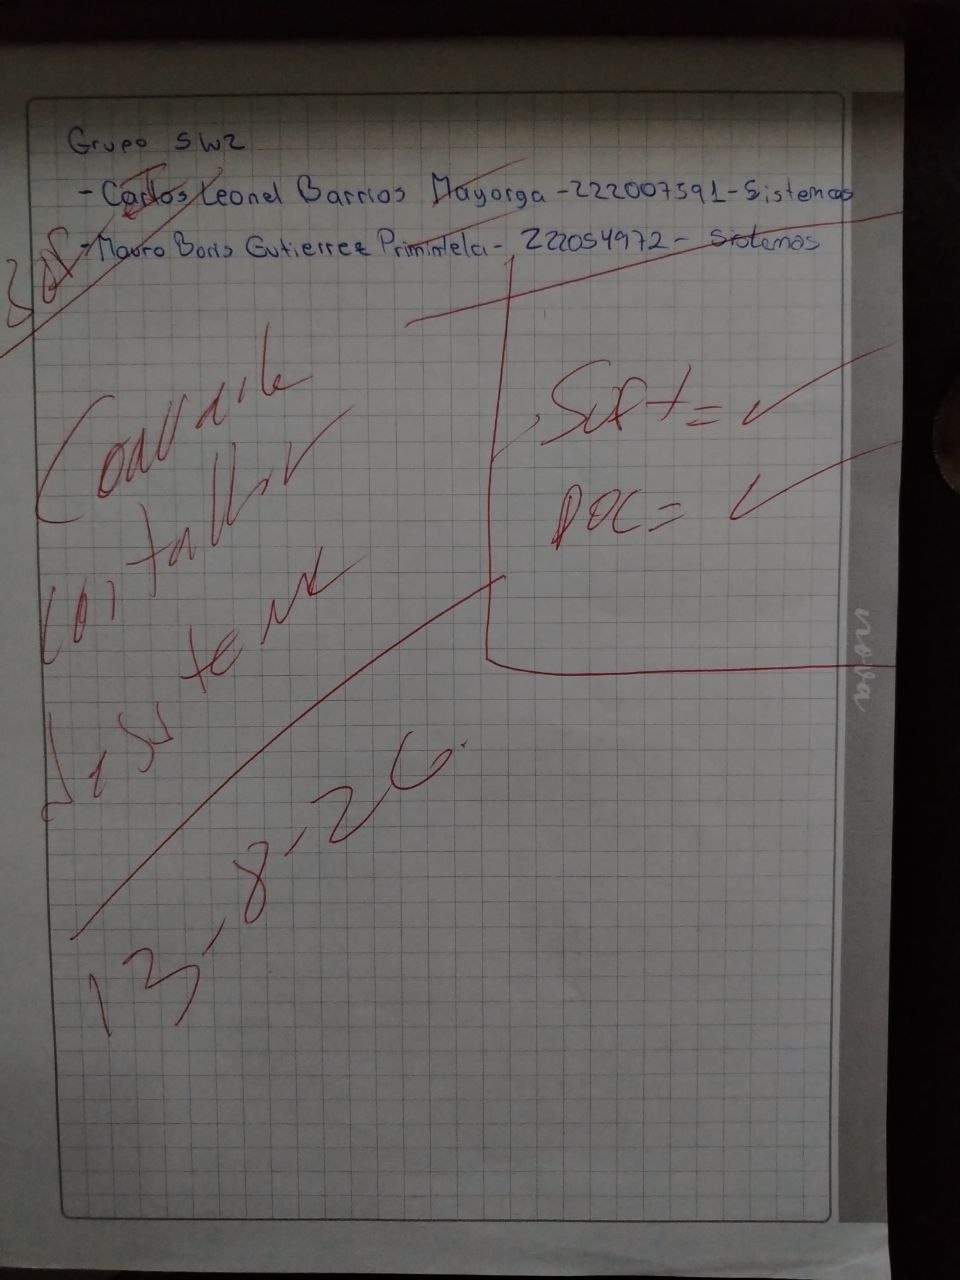
\includegraphics[height=0.62\textheight]{images/170_Hoja_Registro_Grupo_SW2.png}

\smallskip
\noindent\raggedright\textit{Nota.} Elaboración propia. Fotografía de la hoja manuscrita firmada.
\end{figure}

\newpage
\section{Códigos QR}\label{ap:codigos_qr}
\addcontentsline{toc}{section}{Anexo: Códigos QR}

A continuación, se presentan los códigos QR que dan acceso a los recursos del proyecto: el repositorio de código, la carpeta de Google Drive, el sitio web desplegado y el documento.

\begin{figure}[H]
\caption{Códigos QR de los recursos del proyecto}
\label{fig:codigos_qr}
\centering
\begin{tabular}{cc}
    
\includegraphics[width=0.30\textwidth]{images/154_QR_Repositorio.png} &
    
\includegraphics[width=0.30\textwidth]{images/155_QR_GoogleDrive.png} \\
    \small Repositorio de código & \small Carpeta de Google Drive \\[0.5cm]
    
\includegraphics[width=0.30\textwidth]{images/156_QR_Sitio_Desplegado.png} &
    
\includegraphics[width=0.30\textwidth]{images/157_QR_Documento.png} \\
    \small Sitio web desplegado & \small Documento
\end{tabular}

\smallskip
\noindent\raggedright\textit{Nota.} Cada código QR redirige al recurso indicado bajo la imagen.
\end{figure}

\newpage
\section{Estándares de codificación}\label{ap:estandares_codificacion}
\addcontentsline{toc}{section}{Anexo: Estándares de codificación}

Este anexo resume los estándares de codificación aplicados en el repositorio del sistema. Rigen para los tres lenguajes principales del proyecto: Java en el backend, TypeScript en el frontend web y Dart en la aplicación móvil. El módulo de inteligencia artificial, escrito en Python, se rige por su propio linter.

\subsection{Convenciones de nombrado}

Se adopta el estándar propio de cada lenguaje, sin inventar una convención distinta cuando el lenguaje ya tiene una establecida. La Tabla~\ref{tab:estandar_nombrado} resume las reglas.

\begin{table}[H]
\caption{Convenciones de nombrado por lenguaje}
\label{tab:estandar_nombrado}
\begin{threeparttable}
\begin{tabular}{>{\raggedright\arraybackslash}p{3.6cm} >{\raggedright\arraybackslash}p{3.2cm} >{\raggedright\arraybackslash}p{3.8cm} >{\raggedright\arraybackslash}p{3.2cm}}
\toprule
Elemento & Java & TypeScript & Dart \\
\midrule
Variables, funciones y métodos & \texttt{camelCase} & \texttt{camelCase} & \texttt{camelCase} \\
Clases, tipos, interfaces y enumeraciones & \texttt{PascalCase} & \texttt{PascalCase} & \texttt{PascalCase} \\
Constantes & \texttt{UPPER\_SNAKE\_CASE} & \texttt{UPPER\_SNAKE\_CASE} & \texttt{UPPER\_SNAKE\_CASE} \\
Archivos & \texttt{PascalCase.java}, igual al nombre de la clase pública & \texttt{camelCase.ts}; componentes React en \texttt{PascalCase.tsx} & \texttt{snake\_case.dart} \\
\bottomrule
\end{tabular}
\begin{tablenotes}
\item \textit{Nota.} Elaboración propia. En Dart, las constantes de configuración o catálogo del proyecto (códigos de error, claves de almacenamiento) usan \texttt{UPPER\_SNAKE\_CASE} para distinguirlas a simple vista de una variable normal.
\end{tablenotes}
\end{threeparttable}
\end{table}

\subsection{Verificación automática previa al commit}

Las convenciones no dependen de la disciplina individual. La herramienta Husky ejecuta, en cada \texttt{git commit}, el linter que corresponde a los archivos preparados (\textit{staged}) mediante lint-staged. Si el linter detecta un error real, el commit se cancela. La Tabla~\ref{tab:estandar_linters} lista las herramientas por lenguaje.

\begin{table}[H]
\caption{Herramientas de análisis estático por lenguaje}
\label{tab:estandar_linters}
\begin{threeparttable}
\begin{tabular}{>{\raggedright\arraybackslash}p{3.2cm} >{\raggedright\arraybackslash}p{3.6cm} >{\raggedright\arraybackslash}p{6.0cm}}
\toprule
Lenguaje (proyecto) & Herramienta & Alcance y ejecución \\
\midrule
TypeScript (frontend) & ESLint con \texttt{--fix} & Archivos \texttt{.ts} y \texttt{.tsx}; se ejecuta en el pre-commit \\
Java (backend principal) & Checkstyle con configuración propia & Archivos \texttt{.java}; se ejecuta en el pre-commit y se invoca aparte con \texttt{mvn checkstyle:check} \\
Dart (móvil) & \texttt{flutter analyze} con \texttt{flutter\_lints} & Analiza todo el paquete móvil; se ejecuta en el pre-commit \\
Python (módulo de IA) & Ruff (\texttt{ruff check} y \texttt{ruff format}) & No está en el pre-commit; corre en el trabajo \texttt{ia} de la integración continua y en local \\
\bottomrule
\end{tabular}
\begin{tablenotes}
\item \textit{Nota.} Elaboración propia a partir de las reglas del repositorio.
\end{tablenotes}
\end{threeparttable}
\end{table}

La configuración de Checkstyle es propia del proyecto, no la de Google ni la de Sun. Cubre la indentación de cuatro espacios, fijada en el archivo \texttt{.editorconfig}, y las convenciones de nombrado de la Tabla~\ref{tab:estandar_nombrado}. Su regla de nombre de método es más flexible para admitir los nombres de pruebas con el formato \texttt{accion\_condicion\_resultado} (por ejemplo, \texttt{crearUsuario\_conEmailDuplicado\_lanzaConflictException}).

El pre-commit solo aplica el análisis estático y no ejecuta las pruebas. Correr la suite completa (\texttt{pnpm test}, \texttt{./mvnw test} y \texttt{flutter test}) es responsabilidad de cada desarrollador antes de confirmar los cambios, de modo que el hook se mantenga rápido.

\subsection{Formato de los mensajes de commit}

Todo commit sigue el formato \texttt{tipo[SCOPE]: descripción concreta}, validado por \textit{commitlint} mediante el hook \texttt{commit-msg}. Se adaptó la convención de \textit{Conventional Commits}: el alcance va entre corchetes y en mayúsculas, y es obligatorio.

\begin{itemize}
    \item \textbf{Tipos permitidos:} \texttt{feat}, \texttt{fix}, \texttt{refactor}, \texttt{docs}, \texttt{test}, \texttt{chore}, \texttt{style}, \texttt{perf}, \texttt{build} y \texttt{ci}.
    \item \textbf{Alcances válidos:} \texttt{BACK}, \texttt{FRONT}, \texttt{MOBILE}, \texttt{INFRA}, \texttt{DOCS} y \texttt{REPO}.
    \item \textbf{Un commit, un alcance:} un commit nunca toca más de un alcance. Un cambio que afecta al backend y al frontend se divide en dos commits, lo que mantiene el historial legible por módulo y permite revertir un lado sin afectar al otro.
    \item \textbf{Ramas:} las funcionalidades usan \texttt{feature/\{modulo\}}, por ejemplo \texttt{feature/usuarios}.
\end{itemize}

Un ejemplo válido es \texttt{feat[BACK]: Creación de model Usuario}.

\subsection{Convenciones específicas del backend (Java)}

El backend sigue una organización por funcionalidades bajo el paquete \texttt{com.comedoruagrm.backend}, con las carpetas \texttt{common}, \texttt{config}, \texttt{security} y \texttt{features}. Cada módulo de \texttt{features} agrupa sus clases en subcarpetas (\texttt{controller}, \texttt{service}, \texttt{repository}, \texttt{dto}, \texttt{model}, \texttt{mapper}, \texttt{exception} y, si aplican, \texttt{enums}, \texttt{constant} y \texttt{aspect}); ninguna clase queda suelta en la raíz del módulo. Una clase que usa un solo módulo vive en ese módulo, y \texttt{common} se reserva para lo que comparten al menos dos funcionalidades.

\begin{table}[H]
\caption{Nombres de clases del backend}
\label{tab:estandar_clases_java}
\begin{threeparttable}
\begin{tabular}{>{\raggedright\arraybackslash}p{3.6cm} >{\raggedright\arraybackslash}p{5.2cm} >{\raggedright\arraybackslash}p{4.0cm}}
\toprule
Tipo & Convención & Ejemplo \\
\midrule
Controlador & \texttt{\{Recurso\}Controller} & \texttt{UsuarioController} \\
Servicio & \texttt{\{Recurso\}Service}, clase concreta sin interfaz \texttt{Impl} & \texttt{UsuarioService} \\
Repositorio & \texttt{\{Recurso\}Repository} & \texttt{UsuarioRepository} \\
Model (clase mapeada a tabla) & Nombre de dominio en singular, sin sufijo & \texttt{Usuario} \\
DTO de entrada & \texttt{\{Recurso\}Request} o \texttt{Crear\{Recurso\}Request} & \texttt{CrearUsuarioRequest} \\
DTO de salida & \texttt{\{Recurso\}Response} & \texttt{UsuarioResponse} \\
Mapeador & \texttt{\{Recurso\}Mapper} & \texttt{UsuarioMapper} \\
Códigos de error & \texttt{\{Recurso\}ErrorCodes} & \texttt{UsuarioErrorCodes} \\
\bottomrule
\end{tabular}
\begin{tablenotes}
\item \textit{Nota.} Elaboración propia. La clase mapeada a una tabla se llama \textit{Model} en el proyecto, pero conserva la anotación \texttt{@Entity} de JPA por requisito del marco de trabajo.
\end{tablenotes}
\end{threeparttable}
\end{table}

Además, se aplican las siguientes reglas de estilo:

\begin{itemize}
    \item Inyección de dependencias por constructor, mediante \texttt{@RequiredArgsConstructor} de Lombok sobre campos \texttt{private final}.
    \item Los DTO y las clases \texttt{ApiResponse} y \texttt{PageMeta} se definen como \texttt{record} de Java, por ser inmutables y no requerir código repetitivo.
    \item En los Models se usa \texttt{@Getter} a nivel de clase y \texttt{@Setter} solo en los campos que realmente deben mutarse. No se usa \texttt{@Data}, porque \texttt{@ToString} y \texttt{@EqualsAndHashCode} automáticos pueden exponer campos sensibles (como \texttt{passwordHash}) o disparar la carga perezosa en relaciones bidireccionales.
    \item Las enumeraciones persistidas usan \texttt{@Enumerated(EnumType.STRING)}, nunca \texttt{ORDINAL}.
    \item Las anotaciones personalizadas (por ejemplo, \texttt{@CurrentUserId}) se definen una sola vez, en \texttt{security} o en \texttt{common}, y no se duplican entre módulos.
\end{itemize}

\subsection{Comentarios y documentación en el código}

Un comentario explica el \textit{porqué} de una decisión no evidente (una restricción externa, una solución temporal o un comportamiento que sorprendería al lector), y no repite lo que el código ya expresa. Si eliminar el comentario no genera ninguna duda, el comentario sobra.

Dentro de los bloques de documentación (Javadoc, JSDoc y Dartdoc) se usan los prefijos de la extensión \textit{Better Comments} de Visual Studio Code, resumidos en la Tabla~\ref{tab:estandar_comentarios}.

\begin{table}[H]
\caption{Prefijos de comentarios (Better Comments)}
\label{tab:estandar_comentarios}
\begin{threeparttable}
\begin{tabular}{>{\raggedright\arraybackslash}p{4.0cm} >{\raggedright\arraybackslash}p{8.8cm}}
\toprule
Prefijo & Significado \\
\midrule
\texttt{* texto} & Comentario normal \\
\texttt{* * texto} & Información importante a resaltar \\
\texttt{* ! texto} & Alerta, código obsoleto o \textit{no usar} \\
\texttt{* ? texto} & Pregunta abierta o aspecto por revisar \\
\texttt{* TODO: texto} & Tarea pendiente \\
\bottomrule
\end{tabular}
\begin{tablenotes}
\item \textit{Nota.} Elaboración propia a partir de las reglas del repositorio.
\end{tablenotes}
\end{threeparttable}
\end{table}
